\section{Network Access Layer}

% TODO gigabit, 10gigabit, 40/100gigabit ethernet

\subsection{SDU/PDU}

Die Service Data Unit (SDU oder auch Payload) eines Layers ist die Protocol Data
Unit (PDU) des darüberliegenden Layers.

PDU = Protokollinformationen (PCI) + SDU

Layer 1 SDU = Layer 2 PDU


\subsection{Ethernet}

\subsubsection{10Base-T}

\textbf{Wiring}

Transmit (TX) auf Pins 1 und 2\\
Receive (RX) auf Pins 3 und 6

\textbf{Codierung}

Der 10Base-T Standard verwendet Manchester Codierung. Daher ist für 10 Mbit
Datenübertragungsraten eine effektive Übertragungsrate von 20 Mbit erforderlich,
weil für die Codierung eines Bits zwei Signale benötigt werden. Die Bitrate ist
in diesem Fall halb so gross wie die Baudrate.

\textbf{Daten}

Bitdauer:
\[
	\frac{\SI{1}{\second}}{\SI{e7}{\bit}} = \SI{100}{\ns}
\]

Ausbreitung Elektromagnetischer Wellen im Kabel: 
\[
	\frac{2}{3} \cdot 300\cdot \SI{e6}{\meter\per\second} = \SI{0.2}{\meter\per\ns}
\]

Länge eines Bits im Kabel:
\[
	\SI{100}{\ns} \cdot \SI{0.2}{\meter\per\ns} = \SI{20}{\meter}
\]


\subsubsection{100Base-TX}

\textbf{Wiring}

Transmit (TX) auf Pins 1 und 2\\
Receive (RX) auf Pins 3 und 6

\textbf{Codierung}

Der 100Base-TX Standard verwendet eines sogenanntes 4B5B Encoding
(Block-Codierung). Jedes 4 Bit Wort wird auf ein 5 Bit Wort abgebildet, so dass
nie mehr als 3 aufeinander folgende Nullen vorhanden sind. Somit ist eine
sogenannte Symbolrate/Baudrate von +25\%, also 125 Mbps, notwendig.

Um das Übertragene Spektrum zu verkleinern, werden die Bits zusätzlich mittels
MLT-3 (Multi-Level-Transition) Verfahren codiert.

Die Taktrückgewinnung mit reiner MLT-3 Codierung ist nicht möglich, durch die
vorangegangene 4B5B Codierung jedoch schon. Zusätzlich bleiben durch die 4B5B
Codierung weitere $2^5-2^4=16$ Codes übrig, die zur
Synchronisation/Signalisierung verwendet werden können.

\textbf{Daten}

Bitdauer:
\[
	\frac{\SI{1}{\second}}{\SI{e8}{\bit}} = \SI{10}{\ns}
\]

Länge eines Bit im Kabel:
\[
	\SI{10}{\ns} \cdot \SI{0.2}{\meter\per\ns} = \SI{2}{\meter}
\]


\subsubsection{CSMA/CD}

Kollisionen könnnen bei Verwendung von TP-Kabeln nur in Half-Duplex-Mode
Übertragungen auftreten. Im Full-Duplex-Mode werden zwei separate Aderpaare zum
Senden und Empfangen der Daten verwendet, Kollisionen können so physikalisch
nicht auftreten. Kollisionserkennung wird heute also eigentlich nur noch in
Legacy-Netzwerken genutzt.

CSMA mit CD (Collision Detection) verwendet folgenden Algorithmus, um eine
korrekte Übertragung zu ermöglichen:

\textbf{Hauptablauf}

\begin{enumerate}
	\item Ist das Frame bereit zur Übertragung? Wenn ja, gehe zum nächsten
		Schritt.
	\item Ist das Medium frei? Wenn nicht, warte bis es frei ist.
	\item Beginne Übertragung.
	\item Gab es eine Kollision? Wenn ja, starte Kollisionsbehandlung.
	\item Retransmission Counter zurücksetzen und Übertragung beenden.
\end{enumerate}

\textbf{Kollisionsbehandlung}

\begin{enumerate}
	\item Jam-Signal aussenden, damit auch andere Stationen die Kollision erkennen.
	\item Retransmission Counter erhöhen.
	\item Falls die Maximalanzahl Übertragungsversuche erreicht wurde, abbrechen.
	\item Zufällige Wartezeit berechnen (Backoff-Algorithmus), warten.
	\item Hauptablauf erneut beginnen.
\end{enumerate}


\subsubsection{Autonegotiation}

Grundsätzlich kann über Autonegotiation nur der Speed erkannt werden. Der Duplex
Default bei Autonegotiation ist HD.

\begin{tabular}{|c|c|c|c|c|c|c|}
\hline
• & auto & 10 HD & 10 FD & 100 HD & 100 FD & 1000 FD \\
\hline
auto & ok & ok & DM & ok & DM & ok \\
\hline
10 HD & ok & ok & DM & SM & SM & SM \\
\hline
10 FD & DM & DM & ok & SM & SM & SM \\
\hline
100 HD & ok & SM & SM & ok & DM & SM \\
\hline
100 FD & DM & SM & SM & DM & ok & SM \\
\hline
1000 FD & ok & SM & SM & SM & SM & ok \\
\hline
\end{tabular}

DM = Duplex Mismatch, SM = Speed Mismatch.


\subsubsection{MAC-Frame}

Die Minimallänge eines MAC Frames beträgt 64 Bytes, bedingt durch den CSMA/CD
Mechanismus zur Kollisionsdetektion.

Die Maximalgrösse beträgt 1500 Bytes Payload + 12 Bytes SA/DA + 2 Bytes LEN/PT +
4 Bytes Checksum = 1518 Bytes an Daten. Hinzu kommen noch 8 Bytes für Preamble
und SFD.

\begin{center}
	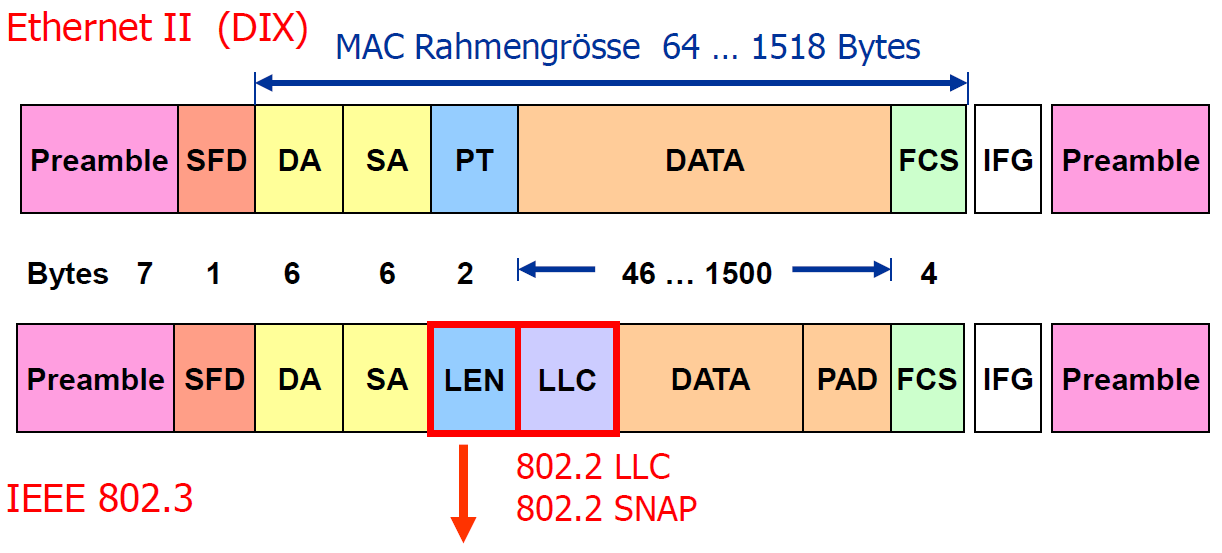
\includegraphics[width=0.8\textwidth]{media/MACFrame.png}
\end{center}

\textbf{Ethernet II}

Ethernet II (DIX) Pakete werden durch einen PT grösser als 1500
(0x05DC) gekennzeichnet. Payloadtype für IP: 0x800, für ARP: 0x806.

\textbf{802.3}

Ethernet 802.3 Pakete sind durch Angaben im LEN Feld kleiner als 1500
gekennzeichnet. Die Länge gibt die PDU Länge des LLC Protokolls an.


\subsection{WLAN}

\subsubsection{Pegelwerte und Dezibel}

Da sich die Pegelunterschiede in der Regel um mehrere 10er Potenzen unterscheiden,
gibt man sie in logarithmischen Massen an.
\[
	\textrm{Pegeldifferenz} = 10 \log (P_1/P_0)~\textrm{dB}
\]
Die Multiplikation mit 10 ergibt sich durch die Umformung von Bel nach Dezibel.
\[
	\textrm{Leistungsverhältnis} = 10^{(\textrm{Pegeldifferenz}/10)}
\]
Nachfolgend einige nützliche Beispielverhältnisse:

\begin{tabular}{|c|c|c|}
	\hline
	\textbf{Leistungsverhältnis} & \textbf{in Dezibel} & \textbf{Berechnung} \\
	\hline
	1 & 0 dB & $10^0=1$ \\
	\hline
	10 & 10 dB & $10^1=10$ \\
	\hline
	100 & 20 dB & $10^2=100$ \\
	\hline
	1000 & 30 dB & $10^3=1000$ \\
	\hline
	2 & 3 dB & $10^0.3=2$ \\
	\hline
\end{tabular}

Andere Leistungsverhältnisse können leicht davon abgeleitet werden durch eine Multiplikation:
\[
	\textrm{Leistungsverhältnis}~8 = 2 \cdot 2 \cdot 2 = 3~\textrm{dB} + 3~\textrm{dB} + 3~\textrm{dB}
\]
Leistungsverhältnisse > 0 sind Verstärkungen, bei Verhältnissen < 0 handelt es sich um Dämpfungen.

In der Praxis ist es gebräuchlich auf die Leistung von 1 mW Bezug zu nehmen.
Dafür verwendet man die Einheit dBm.
\[
	20~\textrm{dBm} = 10 \log (\SI{100}{\milli\watt}/\SI{1}{\milli\watt})
\]


\subsubsection{CSMA/CA}

Im Gegensatz zu Ethernet setzt man im Drahtlos-Bereich statt auf Collision
Detection (CSMA/CD) auf Collision Avoidance (CSMA/CA).

Der Netzadapter ist nicht notwendigerweise Voll-Duplex-fähig. Während einer
eigenen Übertragung kann das Medium nicht überwacht werden. Deshalb würde eine
Collision Detection fehlschlagen. Deswegen wurde CSMA/CD zu einem Mechanismus
weiterentwickelt, der konsequenter dem Prinzip ``listen before talk'' folgt.
Dadurch lassen sich gleichzeitige Datenübertragungen zwar nicht völlig
verhindern, aber doch minimieren.

\begin{center}
	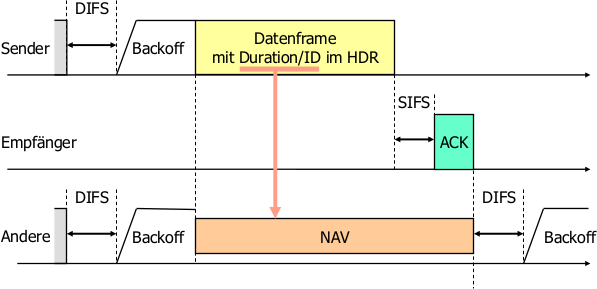
\includegraphics[width=.8\textwidth]{media/csma_ca.png}
\end{center}

\begin{enumerate}
	\item Zuerst wird das Medium abgehört (Carrier Sense).
	\item Ist das Medium für die Dauer eines DIFS (Distributed Coordination
		Function Interframe Spacing) frei, wird eine Backoffzeit aus dem Contention
		Window ausgewürfelt und nach Ablauf dieser gesendet.
	\item Ist das Medium belegt, wird der Backoff bis zum Ablauf des Network
		Allocation Vectors (NAV) gestoppt, bevor er nach einem weiteren DIFS
		entsprechend weiter läuft.
	\item Nach vollständigem Empfang des Paketes wartet der Empfänger ein SIFS
		(Short Interframe Spacing), bevor das ACK gesendet wird.
	\item Eine Kollision durch gleichzeitigen Ablauf des Backoffs führt zu einem
		ACK-Timeout -- nach welchem ein EIFS (Extended Interframe Spacing) gewartet
		wird bevor sich der gesamte Vorgang wiederholen kann (DIFS $\rightarrow$ BO
		\ldots).
\end{enumerate}

Es gilt SIFS < DIFS < EIFS.


\subsubsection{RTS/CTS}

Das RTS/CTS (Request To Send, Clear To Send) Protokoll wird verwendet, um das
``Hidden Station Problem'' zu vermindern. Die volle Bezeichnung lautet
\textit{CSMA/CA RTS/CTS}.

\begin{center}
	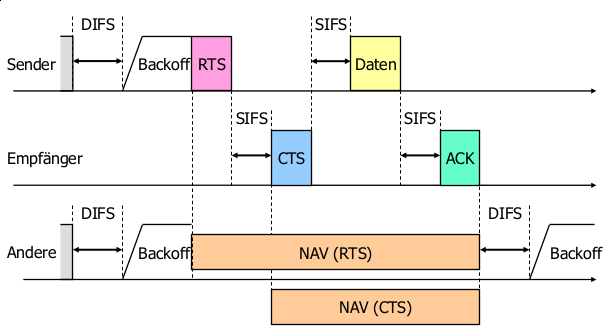
\includegraphics[width=.8\textwidth]{media/rts_cts.png}
\end{center}

Die Sendestation versucht nach Abwarten von DIFS den Kanal mit einem RTS-Paket
für eine bestimmte, in dem Paket angegebene Zeit zu belegen. Der Empfänger
bestätigt dies nach Abwarten von SIFS mit einem CTS-Paket, das ebenfalls eine
Belegungsdauer für den Kanal enthält.

Alle in dem Übertragungsbereich befindlichen Stationen, die dieses RTS
empfangen, schweigen solange, bis die vom Empfänger zurückkommende CTS-Antwort
(clear to send, enthält die Länge des Datenrahmens kopiert aus dem RTS)
konfliktfrei empfangen wurde und die Sendestation die Daten versandt hat.
Entsprechend warten alle Empfänger des CTS entsprechend der im CTS stehenden
Länge.

Falls doch Kollisionen geschehen, wird der binäre exponentielle
Backoff-Algorithmus verwendet, um die Wartezeit zu berechnen.


\subsubsection{Amplitudenmodulation}

% TODO unmatched parentheses, add explanations
\[
	\cos (2\pi \cdot F_N) \cdot \cos (2\pi \cdot F_T)
	= \frac{1}{2}(\cos (2\pi \cdot F_T - 2\pi \cdot F_N)
	+ cos(2\pi \cdot F_T + 2\pi \cdot F_N)
\]

Somit hat sich zum einen die Regellage verschoben und es ist noch eine Kehrlage
hinzugekommen: $\cos (2\pi F_T - F_N)$.


\subsection{ADSL}

ADSL läuft auf über die reguläre Telefon-Kupferleitung (POTS, Plain Old
Telephone Service). Daher kann das Frequenzband von 0~kHz bis 30~kHz nicht
genutzt werden, da dieses durch das Analog-Telefon bereits belegt ist.


\subsection{MAC-Adressen}

Das LSB im ersten Adddress Byte (Most Significant Octet) der Destination Address
ist das Individual/Group Bit.

\begin{tabular}[h]{|l|l|}
	\hline
  \textbf{Value} & \textbf{Address Type} \\
	\hline
  0 & Individual Address \\
  1 & Multicast/Broadcast Address \\
	\hline
\end{tabular}

Das zweite Bit ist das Universal/Local Bit.

\begin{tabular}[h]{|l|l|}
	\hline
  \textbf{Value} & \textbf{Address Type} \\
	\hline
  0 & Globally Administered Address \\
  1 & Locally Administered Address \\
	\hline
\end{tabular}

Die ersten drei Byte der MAC-Adresse werden auch als OUI (Organizationally
Unique Identifier) bezeichnet.


\subsection{Switch Forwarding Methoden}

\begin{center}
	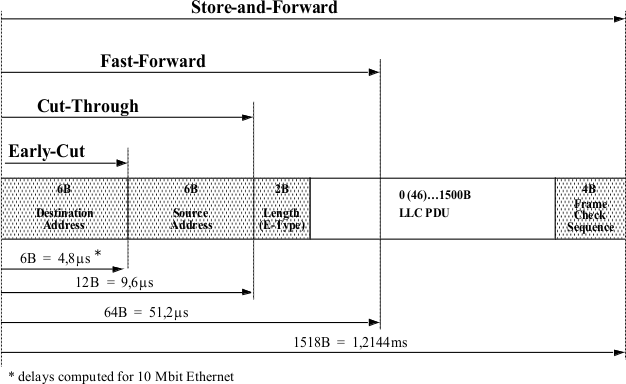
\includegraphics[width=0.8\textwidth]{media/switch_forwarding.png}
\end{center}

\begin{minipage}[t]{.45\linewidth}
	\textbf{Early-Cut}
	\begin{itemize}
		\item Nur nach der Lernphase sinnvoll
		\item Leitet praktisch alle fehlerhaften Frames weiter
	\end{itemize}
\end{minipage}
\hspace{.1\linewidth}
\begin{minipage}[t]{.45\linewidth}
	\textbf{Cut-Through}
	\begin{itemize}
		\item Liest Quell- und Zieladresse
		\item Leitet viele fehlerhafte Frames weiter
	\end{itemize}
\end{minipage}

\begin{minipage}[t]{.45\linewidth}
	\textbf{Fast-Forward}
	\begin{itemize}
		\item Erkennt ``Runts'' (zu kleine Pakete) und Kollisionen
		\item Kann bestimmte EtherTypen filtern
	\end{itemize}
\end{minipage}
\hspace{.1\linewidth}
\begin{minipage}[t]{.45\linewidth}
	\textbf{Store-and-Forward}
	\begin{itemize}
		\item Erkennt CRC-Fehler
		\item Kann Filtering aufgrund von Informationen aus höheren OSI-Schichten
			durchführen
		\item Aufgrund grösserer Delays nicht für Echtzeitsysteme geeignet
	\end{itemize}
\end{minipage}
